\documentclass[12pt]{article}
\usepackage[lmargin=.75in,rmargin=.75in,tmargin=1.in,bmargin=1in]{geometry}
\usepackage{graphicx}
\usepackage{amsmath}
 \usepackage{courier}
\usepackage{listings}
\usepackage{amssymb}
\usepackage{slashbox}
\title{\textbf{CS 760 HW2}}
\author{\textbf{Zhewen Song}}
\begin{document}
%\maketitle
\section*{Part 2}
\subsection*{1}
\begin{center}
	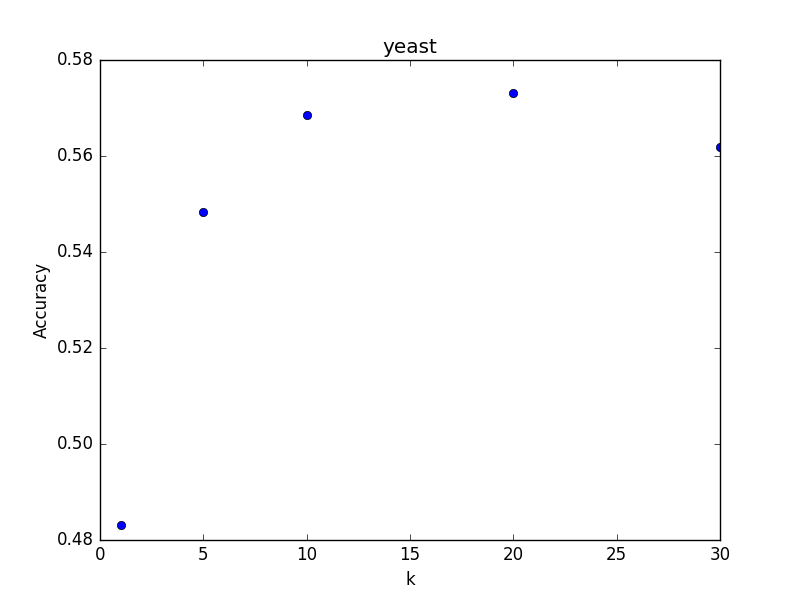
\includegraphics[scale=0.6]{yeast.png}
\end{center}
\subsection*{2}
\begin{center}
	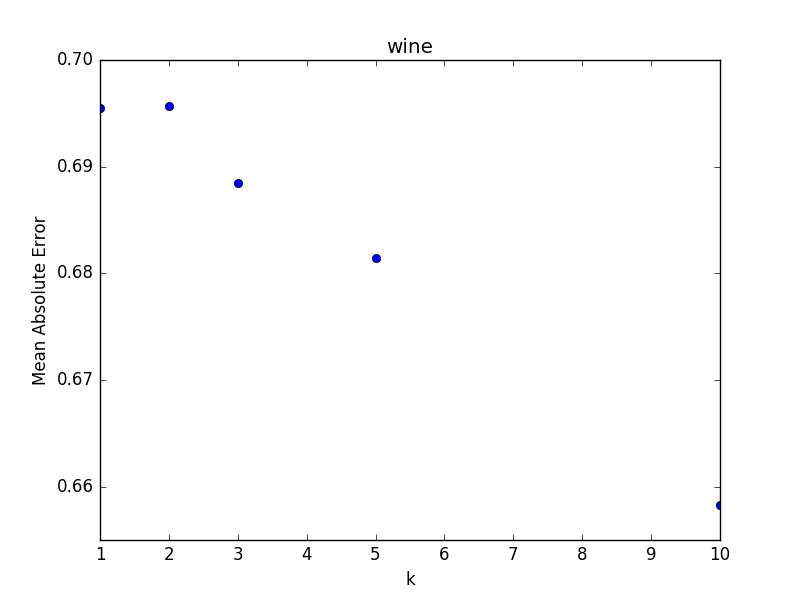
\includegraphics[scale=0.6]{wine.png}
\end{center}
\subsection*{3}
$k=1:$
\begin{center}
	\begin{tabular}{c|cccccccccccc}
	\hline
\backslashbox{Predicted}{Actual} & CYT &NUC& MIT& ME3& ME2& ME1& EXC& VAC& POX& ERL\\
\hline
CYT              & 69& 46& 26&  3&  3&  0&  0&  3&  1&  0\\ 
NUC              & 39& 57& 12&  9&  0&  0&  0&  0&  1&  0\\ 
MIT              & 21& 13& 34&  2&  2&  1&  1&  1&  1&  0\\ 
ME3              &  4&  6&  2& 32&  3&  0&  0&  0&  0&  0\\ 
ME2              &  1&  0&  3&  1&  6&  3&  1&  0&  0&  0\\ 
ME1              &  0&  0&  0&  0&  1&  6&  3&  1&  0&  0\\ 
EXC              &  1&  0&  2&  0&  2&  3&  5&  0&  0&  0\\ 
VAC              &  2&  1&  0&  0&  0&  0&  0&  1&  0&  0\\ 
POX              &  1&  0&  2&  0&  1&  1&  0&  0&  5&  0\\ 
ERL              &  0&  0&  0&  0&  0&  0&  0&  0&  0&  0\\ 
\hline
\end{tabular}\\

\end{center}
$k=30:$
\begin{center}
	\begin{tabular}{c|cccccccccccc}
	\hline
\backslashbox{Predicted}{Actual} & CYT &NUC& MIT& ME3& ME2& ME1& EXC& VAC& POX& ERL\\
\hline
CYT              & 89& 48& 25&  3&  4&  0&  0&  2&  6&  0\\ 
NUC              & 36& 59&  5&  2&  2&  0&  0&  3&  0&  0\\ 
MIT              & 11& 13& 45&  2&  3&  1&  1&  1&  2&  0\\ 
ME3              &  1&  3&  1& 40&  3&  0&  0&  0&  0&  0\\ 
ME2              &  0&  0&  1&  0&  3&  1&  0&  0&  0&  0\\ 
ME1              &  1&  0&  3&  0&  3&  9&  4&  0&  0&  0\\ 
EXC              &  0&  0&  1&  0&  0&  3&  5&  0&  0&  0\\ 
VAC              &  0&  0&  0&  0&  0&  0&  0&  0&  0&  0\\ 
POX              &  0&  0&  0&  0&  0&  0&  0&  0&  0&  0\\ 
ERL              &  0&  0&  0&  0&  0&  0&  0&  0&  0&  0\\ 
\hline
\end{tabular}
\end{center}
Observations:
\begin{itemize}
	\item The correctly classified number of instances for the classes CYT, NUC, MIT, ME3, ME1 \textit{increases} as $k$ increases.
	\subitem We have a large number of instances for these classes, so larger $k$ tends to give a more accurate classification.
	\item The correctly classified number of instances for the classes ME2, EXC, VAC, POX, ERL \textit{does not increase} as $k$ increases.
	\subitem We only have a very limited number of instances for these classes, so larger $k$ does not necessarily yield better result due to the overfitting issue.
\end{itemize}
\section*{Part 3}
\begin{center}
	\begin{tabular}{ccccl}
\hline
pop&	dist&	best dist&	best node&	PQ\\
\hline
-	&$\infty$		&$\infty$			&- &			(f, 0)\\
f	&7.0711&	7.0711&		f&			(h, 0); (c, 1)\\
h	&7.0711&	7.0711&		f&			(i, 0); (c, 1); (g, 5)\\
i	&3	&	3	&		i	&		(c, 1); (j, 3); (g, 5)\\
c	&2	&	2	&		c	&		(e, 0); (b, 0); (j, 3); (g, 5)\\
e	&7.8102	&2	&		c	&		(b, 0); (d, 0); (j, 3); (g, 5)\\
b	&4.4721	&2	&		c	&		(d, 0); (j, 3); (a, 4); (g, 5)\\
d	&5.3852	&2	&		c	&		(j, 3); (a, 4); (g, 5)\\
j   & END WHILE \\
\hline
\end{tabular}
\end{center}
RETURNS c.
\end{document}